% !TEX TS-program = pdflatexmk
\documentclass[12pt]{article}
 \usepackage[margin=1in]{geometry} 
\usepackage{amsmath,amsthm,amssymb,amsfonts}
 \newtheorem{definition}{Definition}[section]
 \newtheorem{theorem}{Theorem}[section]
  \newtheorem{sats}{Sats}[section]
\usepackage[most]{tcolorbox}
\setlength{\parindent}{0.0in}
\setlength{\parskip}{0.05in}
\usepackage{empheq}
\usepackage{float}

\usepackage{framed}
\usepackage[most]{tcolorbox}
\usepackage{xcolor}
\colorlet{shadecolor}{orange!15}
\parindent 0in
\parskip 12pt
\geometry{margin=1in, headsep=0.25in}
\usepackage{amsthm}
\usepackage[utf8x]{inputenc}
\usepackage{comment}
\usepackage{xcolor}
\newcommand{\N}{\mathbb{N}}
\newcommand{\Z}{\mathbb{Z}}
\usepackage{graphicx}
\usepackage{pgf,tikz,pgfplots}
\pgfplotsset{compat=1.15}
\usepackage{mathrsfs}
\usetikzlibrary{arrows}
\usepackage{subcaption}
\pagestyle{empty}
\usepackage{systeme}
\usepackage{pgfplots}
\usepackage{hyperref}
\usepackage{amsthm} 
\newenvironment{solution}
  {\renewcommand\qedsymbol{$\blacksquare$}\begin{proof}[Solution]}
  {\end{proof}}
 
\usepackage[]{algorithm2e}

\newenvironment{problem}[2][Problem]{\begin{trivlist}
\item[\hskip \labelsep {\bfseries #1}\hskip \labelsep {\bfseries #2.}]}{\end{trivlist}}
%If you want to title your bold things something different just make another thing exactly like this but replace "problem" with the name of the thing you want, like theorem or lemma or whatever
\usepackage{mathtools}

%TO HIGHLIGHT USE \hl
\usepackage{xcolor}
\usepackage{soul}
\usepackage{bm}

\usepackage{epigraph}


\usepackage{dirtytalk}

\usepackage{mathtools}
\DeclarePairedDelimiter{\innerprod}\langle\rangle
\newcommand\conjinnerp[2][]{\:\overline{\mkern-4mu\innerprod[#1]{#2}\mkern-4mu}\:}
\usepackage{fancyhdr}
\pagestyle{fancy}
\fancyhf{}
\rhead{Electromagnetic Theory}
\lhead{Kiar Fatah}
\rfoot{Page \thepage}


\numberwithin{equation}{section}

\title{Machine Learning}

\author{Kiar Fatah}

\date{\today}
\begin{document}

\maketitle

\newpage

\tableofcontents 

\newpage
\epigraph{If you can’t explain something in simple terms, you don’t understand it.}{\textit{Richard Feynman }}
\newpage
\section{Lecture 2}
A decision tree is a map of the possible outcomes of a series of related choices.
\begin{figure}[!ht]
 
        \begin{subfigure}{0.5\textwidth}
        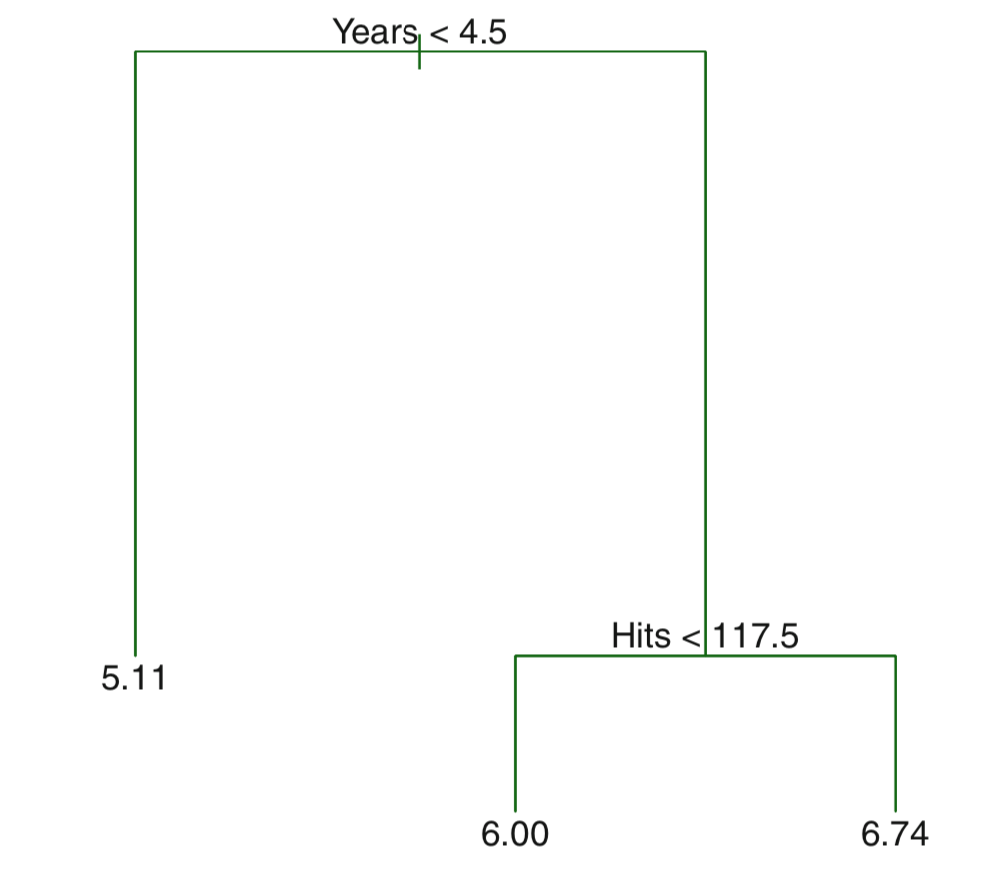
\includegraphics[width=1\linewidth, height=5cm]{decision1.png}
        \caption{A visual map of decision tree.}
        \label{fig:rw}
        \end{subfigure}
        \begin{subfigure}{0.5\textwidth}
        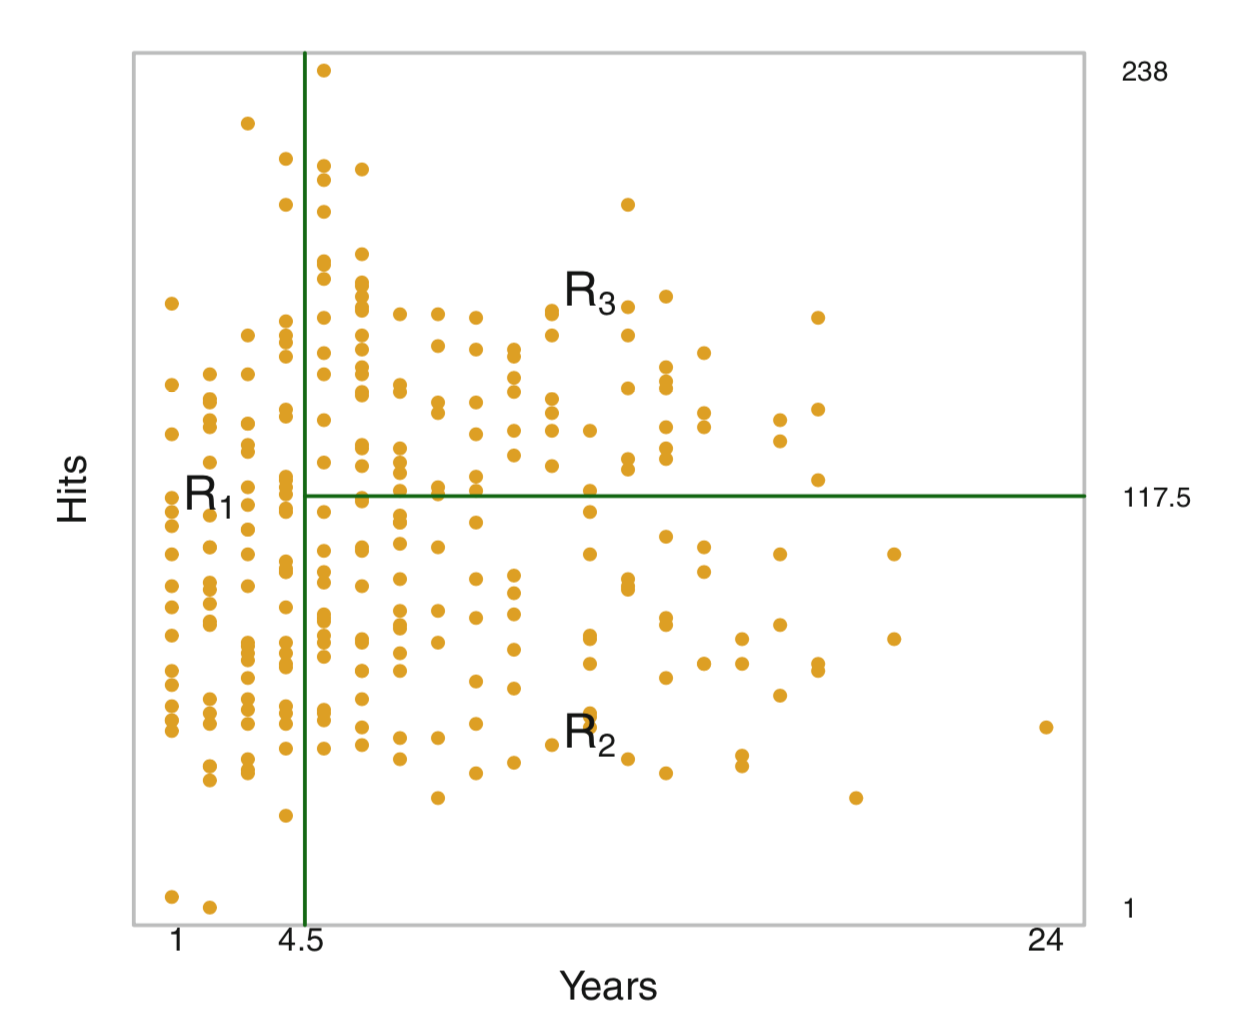
\includegraphics[width=1\linewidth, height=5cm]{decision2.png} 
        \caption{The numerical effect of a decision tree.}
        \label{1}
        
        \end{subfigure}
         
        \caption{}
        \label{fig:image2}
\end{figure}

\subsection{How to ask the best questions?}
The machine will automate the questions for the decision tree, however how does it obtain the best questions to ask? It does so by with the help of Gini impurity and information gain.
\subsubsection{Gini impurity}
Gini impurity is a measurement of uncertainty in a node.It is calculated by how often a randomly chosen element from the set would be incorrectly labeled if it was randomly labeled according to the distribution of labels in the subset. 
\begin{equation}
    1 - \sum_i p_i^2
\end{equation}
\subsubsection{Entropy}
Entropy is also a measurement of uncertainty in a node. It is calculated as
\begin{equation}
    \sum_i -p_ilog_2 p_i
\end{equation}
\subsubsection{Information gain}
Information gain is how much the question reduces the uncertainty. The information is given by the first set of values for the internal node subtracted by the average value of the impurity of the split set. 
\subsubsection{Best question}
The question with the highest value on the information gain will be the one to ask.
\subsubsection{Pruning}
The idea of reduced error pruning is to consider each node in the tree as a candidate for removal. A node is removed if the resulting pruned tree performs at least as well as the original tree over a separate validation dataset.
\subsubsection{Validation set}
Due to pruning there is an need for validation dataset that is not training nor test data set. Therefore if there is access to a rich data set, it is separated to three categories.
\section{Lecture 3}
\subsection{What is Statistical Learning}
We assume that there is some relationship between the output $Y$ and the input $X = X_1, X_2, ...$, that can be written in the general form
\begin{equation}
    Y = f(X) + \epsilon.
\end{equation}
here f is some fixed but unknown function of the input and $\epsilon$ is a random error term, which is independent of the input and has a mean zero. Hence in essence, statistical learning refers to a set of approaches for estimating f.

\subsection{Why Estimate f? }
Two reasons to estimate the unknown function f
\begin{enumerate}
    \item Prediction
    \item Interference
\end{enumerate}
\subsubsection{Prediction}
In common situations a set of inputs are available, however the output can not be easily obtained. In this setting, since the error term averages to zero, the output can be predicted as
\begin{equation}
    \hat{Y} = \hat{f}(X).
\end{equation}
Here $\hat{f}(X)$ represents our estimate for the function f, and $\hat{Y}$ the resulting prediction for the output. Therefore  $\hat{f}(X)$ is treated as a black box, meaning that one is not concerned with the exact form of $\hat{f}$, provided it yields the accurate predictions for the output, Y.

In this case reducible and irreducible error are introduces. Reducible error means $\hat{f}$ is not a perfect estimate for the function f. This will introduce error, however this error is reducible and can be improved. Irreducible error cannot be improved and is introduced by $\epsilon$.
\subsubsection{Inference}
Often one is interested in knowing how the output is affected as the input variables change. The goal is to estimate f but not necessarily to predict Y. Hence $\hat{f}$ can not be treated as a black box. because it is needed to know the exact form. In this case the following questions needs answers
\begin{enumerate}
    \item Which predictors are associated with the response?
    \item What is the relationship between the response and each predictor?
    \item Can the relationship between Y and each predictor be adequately summarized using a linear equation, or is the relationship more complicated?
\end{enumerate}
\subsection{How Do We Estimate f?}
We wanna find a function $\hat{f}$ such that $Y \approx \hat{f}(X)$ for any observation (X,Y). Most statistical learning methods for this task can be characterized as either parametric or non-parametric.
\subsubsection{Parametric Methods}
In parametric methods there is a two-step model-based approach
\begin{enumerate}
    \item Make an assumption about the functional form, or shapre, of f
    \item After a model has been selected, there is a need for a procedure that uses the training data to fit or train the model.
\end{enumerate}
In other words it reduces the problem of estimating f down to one of estimating a set of parameters. The potential disadvantage of a parametric approach is that the model that is chosen will often not match the true unknown form of f. This can be improved by choosing flexible models that can fit many different possible functional forms for f, however it requires a greater number of parameters. Greater number of parameters leads to more complex models that can result in overfitting the data, which means the approximation follows the errors, or noise, too closely.
\subsubsection{Non-parametric Methods}
Non-parametric methods do not make explicit assumptions about the functional form of f . Instead they seek an estimate of f that gets as close to the data points as possible without being too rough or wiggly. Such approaches can have a major advantage over parametric approaches: by avoiding the assumption of a particular functional form for f, they have the potential to accurately fit a wider range of possible shapes for f. Any parametric approach brings with it the possibility that the functional form used to estimate f is very different from the true f, in which case the resulting model will not fit the data well. In contrast, non-parametric approaches completely avoid this danger, since essentially no assumption about the form of f is made. But non-parametric approaches do suffer from a major disadvantage: since they do not reduce the problem of estimating f to a small number of parameters, a very large number of observations (far more than is typically needed for a parametric approach) is required in order to obtain an accurate estimate for f.
\subsection{Assessing Model Accuracy}
In statistical learning there is not one model that dominates over all other models.
\subsection{Measuring the Quality of Fit}
The way to evaluate the performance of a statistical learning methods on a given data set, is through mean squared error (MSE) given by
\begin{equation}
    MSE = \frac{1}{n} \sum_{i = 1}^{n}(y_i-\hat{f}(x_i))^2
\end{equation}
The MSE can be calculated for the training and the test set, however the interest lies in the accuracy of the model on unseen data, test set. Therefore the method that gives the lowest test MSE is the one to choose.

Note that there is no guarantee that the method with the lowest training MSE will also have the lowest test MSE. When a given method yields a small training MSE but a large test MSE, we are said to be overfitting the data. This is due to the model is trying to hard to find patterns in the data but picks up patterns that are caused by chance rather than by true properties.

\subsection{Curse of Dimensionality}
\begin{enumerate}
    \item Easy problems in low-dimensions are harder in high-dimensions
    \item In high-dimensions everything is far from everything else, this is an issue in the nearest neighbour model
    \item Any method that attempts to produce locally varying functions in small isotropic neighbourhoods will run into problems in high dimensions.
\end{enumerate}
\subsection{The Bias-Variance Trade Off}
Let us imagine we could repeat the modeling for many times – each time by gathering new set of training samples, D. The resulting models will have a range of predictions due to randomness in the underlying data set.
\begin{enumerate}
    \item Variance: Refers to the amount by which $\hat{f}$ would change if we estimated it using a different training data set.
    \item Bias: Refers to the error that is introduced by approximating a real-life problem, which may be extremely complicated, by a much simpler model.
\end{enumerate}
This can be showcased in figure \ref{var_bias}
\begin{figure}[!ht]
    \centering
    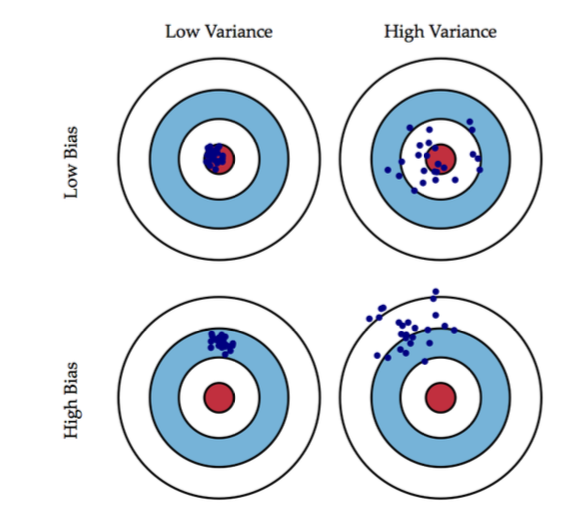
\includegraphics[scale = 0.7]{var_bias.png}
    \caption{Variance versus Bias}
    \label{var_bias}
\end{figure}
In essence the relationship betewen complexity, bias and variance can be summarized as
\begin{enumerate}
    \item Low model complexity implies high bias, low variance.
    \item High model complexity implies low bias, high variance.
\end{enumerate}
A low model complexity can be a decision tree with a low level depth and a high model complexity can be a decision tree with a high level depth.
\subsection{The Validation Set Approach}
The resulting validation set error rate provides an estimate of the test error rate.
\section{Lecture 4}
\subsection{Linear Regression, A Parametric Method}
Simple linear regression assumes theres a linear relationship between the output and input. Hence in the as mention earlier in the section parametric methods, a linear equation is guessed. However, in practice the coefficients are unknown and therefore needs to be approximated. The most common approach is done by least squared method.
\subsection{RANdom SAmpling Consensus}
Random sampling consensus or RANSAC is applied when the data set S contains outliers
\begin{enumerate}
    \item Randomly select a (minimum number of) sample of s data
    points from S and instantiate the model from this subset.
    \item Determine the set of data points $S_i$ which are within a distance threshold t of the model. The set $S_i$ is the consensus set of samples and defines the inliers of S.
    \item If the subset of $S_i$ is greater than some threshold T, re-estimate the model using all the points in Si and terminate
    \item If the size of $S_i$ is less than T, select a new subset and repeat the above.
    \item After N trials the largest consensus set $S_i$ is selected, and the model is re-estimated using all the points in the subset $S_i$
\end{enumerate}
\subsection{Disadvantages with RANSAC}
\subsection{Differences with Parametric and Non-parametric Methods}
\begin{enumerate}
    \item If the parametric form is close to the true form of f, the parametric approach will outperform the non-parametric
    \item As a general rule, parametric methods will tend to outperform non-parametric when there is a small number of observations per predictor (i.e. in a high dimension).
    \item Interpretability stand point: Linear regression preferred to KNN if the test MSEs are similar or slightly lower.
\end{enumerate}
\subsection{k-NN Regression, A Non-parametric}
The k-NN regression method is closely related to the k-NN classifier. Given a value for K and a prediction point $x_0$, k-NN regression first identiffies the K training observations that are closest to $x_0$ represented by $N_0$. It then estimates $f(x_0)$ usin the average of all the training responses in $N_0$. In other words
\begin{equation}
    \hat{f(x_0)} = \frac{1}{K} \sum_{x_i \in N_0} y_i.
\end{equation}
Note larger values of k provide a smoother and less variable fit (lower variance!)
\subsection{Parametric or Non-parametric Methods?}
\begin{enumerate}
    \item  If the parametric form is close to the true form of f, the parametric approach will outperform the non-parametric
    \item As a general rule, parametric methods will tend to outperform non-parametric when there is a small number of observations per predictor (i.e. in a high dimension).
    \item Interpretability stand point: Linear regression preferred to KNN if the test MSEs are similar or slightly lower.
\end{enumerate}
\subsection{Shrinkage Methods}
A common way to fit models is by appling least square, however an alternative is it is possible to fit a model containing all p predictors using a technique that constrains or regularizes the coefficient estimates, or equivalently that shrinks the coefficient estimates towards zero.
\begin{enumerate}
    \item Among a large number of variables X in the model there are generally many that have little (or no) effect on Y
    \item Leaving these variables in the model makes it harder to see the big picture, i.e. the effect of the “important variables”
    \item Would be easier to interpret the model by removing unimportant variables (setting the coefficients to zero)
\end{enumerate}
\subsection{Ride Regression}
Similar to least squares but minimizes different quantity
\begin{enumerate}
    \item Shrinkage penalty
    \item The parameter $\lambda$
    \item Interpation of the graphs
    
\end{enumerate}
\subsection{The Lasso}
Similar to ridge regression but with slightly different term
\section{Lecture 5}
\subsection{Probability Theory in Machine Learning}
The advantages are
\begin{enumerate}
    \item Interpretability: It can be more transparent and mathematically rigorous than other machine learning methods.
    \item Transparency: Assumptions can be made more explicit than in other methods.
    \item Efficiency: It can work in regimes that are data poor.
    \item Flexibility: Easy to merge different parts of a complex system and to update current knowledge with new observations.
    \item Encompassing: Aspects of learning and inference can be cast under the same theory.
\end{enumerate}
The disadvantages are
\begin{enumerate}
    \item Complicated: Often hard to derive closed solutions. Need to resort to computation and heuristic approximations.
    \item Scalability: Not computationally scalable to large dataset.
\end{enumerate}
\subsection{Axiomatic definition of probabilities}
Given an sample space $\omega$ of all possible outcomes, and an event E, or set of outcomes from $\omega$ then
\begin{enumerate}
    \item $P(E) \geq 0$ for all $E \subseteq \omega$.
    \item If $E = \omega$ then the probability of $\omega$ is one. In other words the probability that one event will occur is equal to one.
    \item if the events are a ocuntable sequence of pairwise disjoint events then the probability of the union of each event is equal to the probability of the summation of every event.
\end{enumerate}
\subsection{Random (Stochastic) Variables}
A random variale is neither random nor a variable, it is a function that does exactly what we need, $X: \omega \to \mathcal{R}$.
The probability distribution function, so called pdf, of a random variable maps the range to positive numbers, $Pr(x): X \to \mathbb{R}_{>0}$.
\begin{enumerate}
    \item The probability of a random variables describes how the probability density is distributed over the range of X,
    \begin{equation}
        P[0 \leq X \leq 1] = \int_{x = 0}^1 Pr(x) dx.
    \end{equation}
    \item X is distrubted Pr(x) is written ore compactly as 
    \begin{equation}
        X \tilde Pr(x).
    \end{equation}
\end{enumerate}
\subsection{Types of Random Variables}
\begin{enumerate}
    \item Discrete random variable: Countable set
    \item Continuous random variable: Uncountable set
\end{enumerate}
\subsection{Joint Probabilities}
Consider two random variables X and Y. Observe multiple paired instances, some paried outcomes will occur frequently. This information is encoded in the joint probability density function $Pr(x,y)$.
\subsection{Marginalization}
The probability distribution function, PDF, of any single variable can be recovered from a joint distribution by summin for the discrete case and integrating for the continuous case.
\begin{equation}
    Pr(x) = \sum_y Pr(x,y), (Discrete)
\end{equation}
\subsection{Conditional Probabilities}
The conditional probability of X given that Y takes a value y gives
\begin{equation}
    P(A|B) = \frac{P(A , B)}{P(B)}.
\end{equation}
If it turns out the events are independent then
\begin{equation}
    P(A|B) = \frac{P(A) P(B)}{P(B)}.
\end{equation}
Bayes's theorem gives us
\begin{equation}
    P(A | B) = P(A|B)P(B) = P(B|A)P(A) \implies P(A|B) = \frac{P(B|A) P(A) }{P(B)}.
\end{equation}
\subsection{Common Distributions}
\begin{enumerate}
    \item Bernoulli: Binary variables
    \item Categorical: Discrete variables
    \item Gaussian: Univariate normal distrubtion
\end{enumerate}
\subsection{Central Limit Theorem}
The distribution of a linear combination of a large number of
independent, identically distributed (iid) variables will tend to
normal, regardless of the underlying distribution.1
\subsection{Expectation}
The expected value can be calculated according
\begin{equation}
    \mathbb{E}[X] = \mu_X = \int x Pr(x) dx
\end{equation}
it is equal to the center of gravity of a distribution.

The variance is
\begin{equation}
    Var[X] = \sigma_X^2 = \mathbb{E}[X-\mathbb{E}[X])^2]
\end{equation}
It is interpreted as the spread of a distribution.

Covariance is given by
\begin{equation}
    \sigma_{X,Y} = \mathbb{E}[X-\mathbb{E}[X]](Y-\mathbb{E}[Y])]
\end{equation}
Shows how two variables vary together.
\subsection{General Machine Learning Problem}
if Y is discrete then it is classification, if it is continuous it is regression.
\begin{enumerate}
    \item Learning: We estimate Pr($\bm{x}$, y) from data.
    \item Inference: We estimate Pr(y| $\bm{X} = \bm{x}$) from data.
\end{enumerate}
\subsection{Bayes's Rule}
\begin{enumerate}
    \item $Pr(\bm{x} | Y = y)$: Likelihood represents the probability density of observing data $\bm{x}$ given the hypothesis Y = y
    \item $Pr(Y = y)$: Prior repreents the knowledge about Y before any observation.
    \item $Pr(y | \bm{X} = \bm{x})$: Posterior represents the probabiltiy density of hypothesis y given observation $\bm{X} = \bm{x}$.
    \item $Pr(\bm{X} = \bm{x})$: Evidence describes how well the model fits the evidence.
\end{enumerate}

\end{document}